\documentclass[notes,11pt, aspectratio=169]{beamer}

\usepackage{pgfpages}
% These slides also contain speaker notes. You can print just the slides,
% just the notes, or both, depending on the setting below. Comment out the want
% you want.
\setbeameroption{hide notes} % Only slide
%\setbeameroption{show only notes} % Only notes
%\setbeameroption{show notes on second screen=right} % Both

\usepackage{helvet}
\usepackage[default]{lato}
\usepackage{array}
\usepackage{tgbonum}

\usepackage{tikz}
\usepackage{verbatim}
\setbeamertemplate{note page}{\pagecolor{yellow!5}\insertnote}
\usetikzlibrary{positioning}
\usetikzlibrary{snakes}
\usetikzlibrary{calc}
\usetikzlibrary{arrows}
\usetikzlibrary{decorations.markings}
\usetikzlibrary{shapes.misc}
\usetikzlibrary{matrix,shapes,arrows,fit,tikzmark}
\usepackage{amsmath}
\usepackage{mathpazo}
\usepackage{hyperref}
\usepackage{lipsum}
\usepackage{multimedia}
\usepackage{graphicx}
\usepackage{multirow}
\usepackage{graphicx}
\usepackage{dcolumn}
\usepackage{bbm}
\newcolumntype{d}[0]{D{.}{.}{5}}

\usepackage{changepage}
\usepackage{appendixnumberbeamer}
\newcommand{\beginbackup}{
   \newcounter{framenumbervorappendix}
   \setcounter{framenumbervorappendix}{\value{framenumber}}
   \setbeamertemplate{footline}
   {
     \leavevmode%
     \hline
     box{%
       \begin{beamercolorbox}[wd=\paperwidth,ht=2.25ex,dp=1ex,right]{footlinecolor}%
%         \insertframenumber  \hspace*{2ex} 
       \end{beamercolorbox}}%
     \vskip0pt%
   }
 }
\newcommand{\backupend}{
   \addtocounter{framenumbervorappendix}{-\value{framenumber}}
   \addtocounter{framenumber}{\value{framenumbervorappendix}} 
}


\usepackage{graphicx}
\usepackage[space]{grffile}
\usepackage{booktabs}
\newcommand\independent{\protect\mathpalette{\protect\independenT}{\perp}}
\def\independenT#1#2{\mathrel{\rlap{$#1#2$}\mkern2mu{#1#2}}}
\DeclareMathOperator{\Supp}{Supp}

% These are my colors -- there are many like them, but these ones are mine.
\definecolor{blue}{RGB}{0,114,178}
\definecolor{red}{RGB}{213,94,0}
\definecolor{yellow}{RGB}{240,228,66}
\definecolor{green}{RGB}{0,158,115}

\hypersetup{
  colorlinks=false,
  linkbordercolor = {white},
  linkcolor = {blue}
}


%% I use a beige off white for my background
\definecolor{MyBackground}{RGB}{255,253,218}

%% Uncomment this if you want to change the background color to something else
%\setbeamercolor{background canvas}{bg=MyBackground}

%% Change the bg color to adjust your transition slide background color!
\newenvironment{transitionframe}{
  \setbeamercolor{background canvas}{bg=yellow}
  \begin{frame}}{
    \end{frame}
}

\setbeamercolor{frametitle}{fg=blue}
\setbeamercolor{title}{fg=black}
\setbeamertemplate{footline}[frame number]
\setbeamertemplate{navigation symbols}{} 
\setbeamertemplate{itemize items}{-}
\setbeamercolor{itemize item}{fg=blue}
\setbeamercolor{itemize subitem}{fg=blue}
\setbeamercolor{enumerate item}{fg=blue}
\setbeamercolor{enumerate subitem}{fg=blue}
\setbeamercolor{button}{bg=MyBackground,fg=blue,}



% If you like road maps, rather than having clutter at the top, have a roadmap show up at the end of each section 
% (and after your introduction)
% Uncomment this is if you want the roadmap!
% \AtBeginSection[]
% {
%    \begin{frame}
%        \frametitle{Roadmap of Talk}
%        \tableofcontents[currentsection]
%    \end{frame}
% }
\setbeamercolor{section in toc}{fg=blue}
\setbeamercolor{subsection in toc}{fg=red}
\setbeamersize{text margin left=1em,text margin right=1em} 

\newenvironment{wideitemize}{\itemize\addtolength{\itemsep}{10pt}}{\enditemize}

\usepackage{environ}
\NewEnviron{videoframe}[1]{
  \begin{frame}
    \vspace{-8pt}
    \begin{columns}[onlytextwidth, T] % align columns
      \begin{column}{.70\textwidth}
        \begin{minipage}[t][\textheight][t]
          {\dimexpr\textwidth}
          \vspace{8pt}
          \hspace{4pt} {\Large \sc \textcolor{blue}{#1}}
          \vspace{8pt}
          
          \BODY
        \end{minipage}
      \end{column}%
      \hfill%
      \begin{column}{.38\textwidth}
        \colorbox{green!20}{\begin{minipage}[t][1.2\textheight][t]
            {\dimexpr\textwidth}
            Face goes here
          \end{minipage}}
      \end{column}%
    \end{columns}
  \end{frame}
}

\title[]{\textcolor{blue}{Canonical Research Designs II:\\ Difference-in-Differences II:\\
  Event Studies, Synthetic Control, and Synthetic DinD}}
\author[PGP]{}
\institute[FRBNY]{\small{\begin{tabular}{c}
  Paul Goldsmith-Pinkham  \\
\end{tabular}}}

\date{\today}

\begin{document}

%%% TIKZ STUFF
\tikzset{   
        every picture/.style={remember picture,baseline},
        every node/.style={anchor=base,align=center,outer sep=1.5pt},
        every path/.style={thick},
        }
\newcommand\marktopleft[1]{%
    \tikz[overlay,remember picture] 
        \node (marker-#1-a) at (-.3em,.3em) {};%
}
\newcommand\markbottomright[2]{%
    \tikz[overlay,remember picture] 
        \node (marker-#1-b) at (0em,0em) {};%
}
\tikzstyle{every picture}+=[remember picture] 
\tikzstyle{mybox} =[draw=black, very thick, rectangle, inner sep=10pt, inner ysep=20pt]
\tikzstyle{fancytitle} =[draw=black,fill=red, text=white]
%%%% END TIKZ STUFF

% Title Slide
\begin{frame}
\maketitle
\end{frame}

\begin{frame}{Today's Topics}
  \begin{wideitemize}
  \item Today, touching on two (related) topics
  \item First, finishing up conversation related to last class and
    diff-in-diff, focusing again on discussion of \emph{event studies}
    \begin{itemize}
    \item Focusing on how event studies generate a counteractual
      control unit
    \end{itemize}
  \item Second, discuss synthetic control (and dind) methods
    \begin{itemize}
    \item Not completely new methods, but big upswing in research
    \end{itemize}
  \end{wideitemize}
\end{frame}

\begin{frame}{Event study}
  \begin{columns}[T] % align columns
    \begin{column}{0.7\textwidth}
      \begin{wideitemize}
      \item When we see the event happen and need a control group
      \item Distinguish between event study and diff-in-diff
        \begin{itemize}
        \item What do I view as the diff?
        \item Talk about my exmaple in my paper
        \item Remember what the key identifying assumption is: parallel trends
        \end{itemize}
      \item Key issue is what can identify without more assumptions
      \item Without a true control group, can't have both time fe,   unit fe and the full non-parametric spec. Why?
        \begin{equation}
          Y_{it} = \alpha_{i} + \gamma_{t} + \sum_{s = L_{0}, s\not=-1}^{L_{1}}\underbrace{1(t-T_{i} = s)}_{\text{time periods $s$ before and after treatment}}\mu_{s}
          \end{equation}
        \item Need to exclude both the baseline period AND at least some periods outline the treatment window (e.g. before $L_{0}$ and after $L_{1}$
        \end{wideitemize}
      \end{column}%
      \hfill%
      \begin{column}{.3\textwidth}
        Picture from NOtow paper
      \end{column}%
    \end{columns}
  \end{frame}

\begin{frame}
  \begin{wideitemize}
  \item Our assumptions is the same (or similar) what we discussed last class
    \begin{itemize}
    \item Parallel trends -- but amongst who?
    \item Turns out, all of the groups need to be parallel.
    \item That might be an awful assumption (e.g. very far apart from
      one another)
    \end{itemize}
  \item Sun and Abraham (2020) point out that heterogeneity in
    treatment effects can have big impacts as well
    \begin{itemize}
    \item In fact, it can violate the pre-trend test
    \item The use of ``excluded'' periods potentially contaminates pre-periods
    \item Solution: use ``late'' adopters as control group. 
    \end{itemize}
    \item   Addditional untestable assumptions are required as we allow for more types of heterogeneity
  \end{wideitemize}
\end{frame}

\begin{frame}
  \begin{wideitemize}
  \item   Issue here was the attempt to get a ``free lunch'' -- we always need a control group
  \item   Think back to cross-sectional setting with ATT
    \begin{itemize}
    \item We always knew $Y_{i}(1)$. Key issue is an estimator for $Y_{i}(0)$.
    \item Event study approaches had issues by ignoring this point and hoping regression would solve problem
    \item Notably, this problem disappears if we have full homogeneity + no anticipation and only exclude pre-periods
    \end{itemize}
  \item Point of emphasis -- we need parallel trends to hold to
    construct a counterfactual in these settings. Why?
    $Y_{jt}(0) - Y_{j,t-1}(0)$ needs to be a good approximator of
    $Y_{i,t}(0) - Y_{i,t-1}(0)$.
    \begin{itemize}
    \item Since we imposed
      $Y_{it} = \alpha_{i} + \gamma_{t} + D_{it}\tau$, the first
      differencing makes them good approximations
    \end{itemize}
  \end{wideitemize}
\end{frame}Q

\begin{frame}{Synthetic Control}
  \begin{columns}[T] % align columns
    \begin{column}{0.9\textwidth}
      \begin{wideitemize}
      \item Pivoting slightly: instead of imposing the parallel trends
        assumption directly through the linear model, we could
        construct a combination of units to approximate $Y_{it}(0)$
        \begin{itemize}
        \item This is what one does in the cross-sectional setting with a
          pscore method! E.g. consider the ATT:
          \begin{equation*}
            \tau_{ATT} = \underbrace{Y(1)}_{\text{Fully observed}} - \underbrace{\hat{Y}(0)}_{\text{Constructed}}
          \end{equation*}
        \end{itemize}
      \item How would one pick? Recall that with p-score methods or
        regression, weights effectively reweight based on
        comparability to treated group
        \begin{itemize}
        \item With panel data, can use pre-treatment data to construct
          these weights
        \item This method is known as synthetic control
        \end{itemize}
      \end{wideitemize}
    \end{column}%
    \hfill%
    \begin{column}{.5\textwidth}
    \end{column}%
  \end{columns}
\end{frame}


\begin{frame}{Synthetic Control example - Abadie }
  \begin{columns}[T] % align columns
    \begin{column}{0.5\textwidth}
      \begin{wideitemize}
      \item Consider following problem: California bans smoking in 1989. What does that do to smoking?
        \begin{enumerate}
        \item Define estimand
        \item How can we get at it?
        \end{enumerate}
      \item 
        \end{wideitemize}
    \end{column}%
    \hfill%
    \begin{column}{.5\textwidth}
      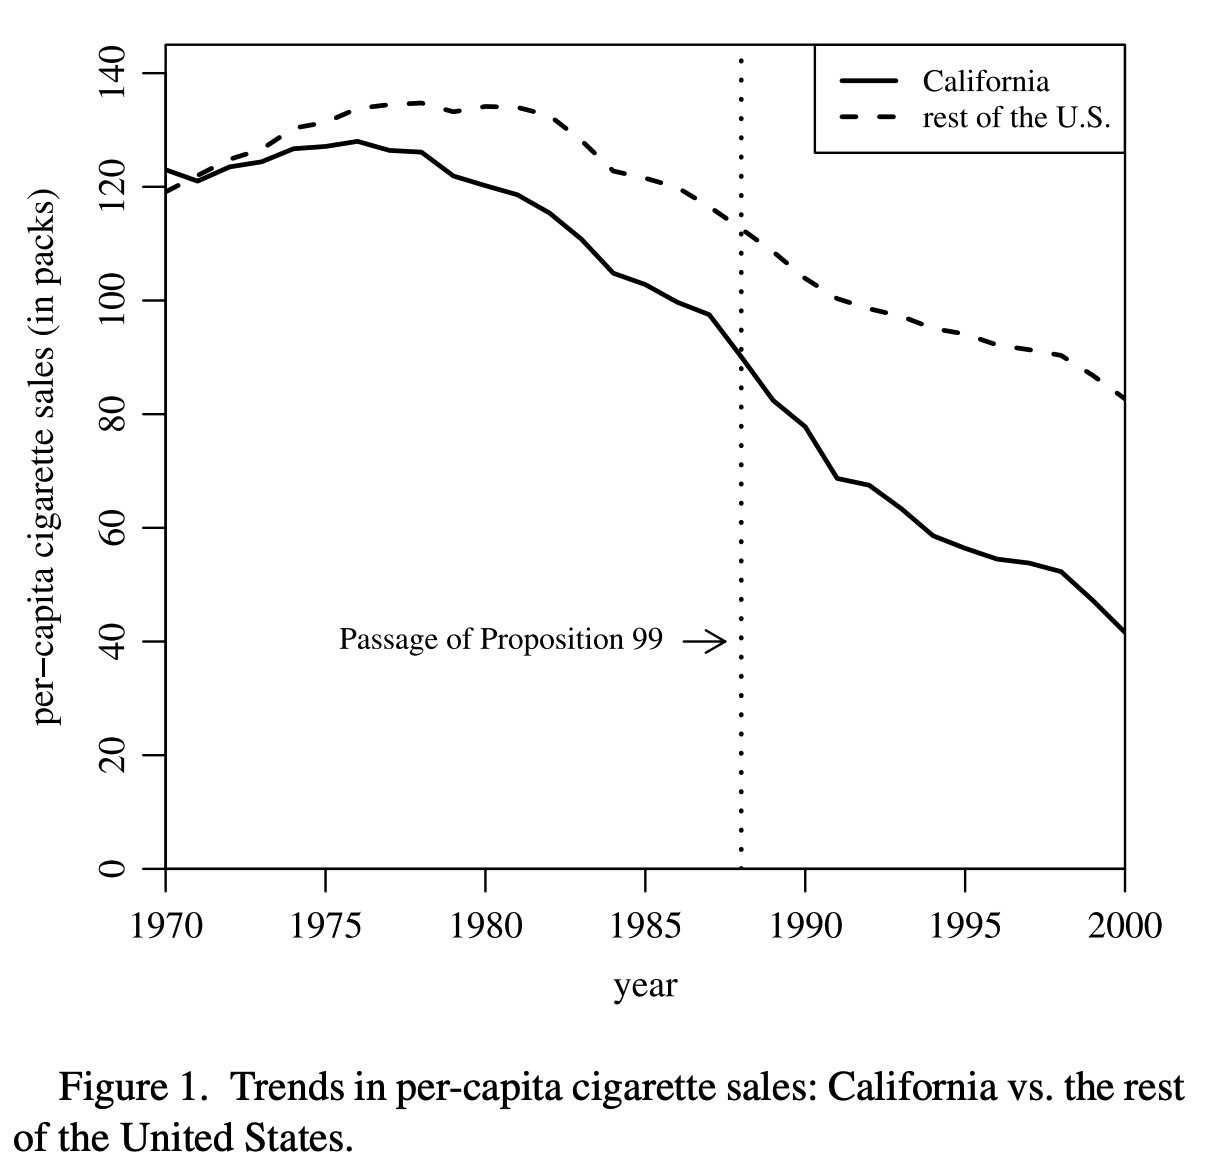
\includegraphics[width=\linewidth]{images/abadie2010a.png}
    \end{column}%
  \end{columns}
\end{frame}


\begin{frame}{Generalized Estimation approach (Doudchenko and Imbens (2018))}

  \begin{wideitemize}
  \item Consider the following general problem
    \item We have a panel with $T$ time periods and $N+1$
      units. Intervention $D_{it}$ at time $T_{0}$ for one unit (unit $i = 0$)
    \item Potential outcomes $Y_{it}(D_{it})$, and we only observe one
      of the potential outcomes (as per usual)
      \begin{itemize}
      \item Fundamental problem of causal inference
      \item We can also have fixed characteristics $X_{it}$
      \end{itemize}
    \item Let $\mathbf{Y}_{a,b}$ denote the vector (or matrix in
      control case) for $a \in \{\text{treatment}, \text{control}\}$ and
      $b \in \{\text{pre}, \text{post}\}$ for the treated and control
      groups in the pre or post period.
    \item Then, we have observations (analogous setup for the covariates):
      \begin{equation*}
        \mathbf{Y} = \left( \begin{array}{cc}
                              \mathbf{Y}_{t,post} & \mathbf{Y}_{c,post} \\
                              \mathbf{Y}_{t,pre} & \mathbf{Y}_{c,pre} \\
                            \end{array}
                            \right) =  \left( \begin{array}{cc}
                              \mathbf{Y}_{t,post}(1) & \mathbf{Y}_{c,post}(0) \\
                              \mathbf{Y}_{t,pre}(0) & \mathbf{Y}_{c,pre}(0) \\
                            \end{array}
                            \right) 
      \end{equation*}
  \end{wideitemize}
\end{frame}

\begin{frame}
        \begin{equation*}
        \mathbf{Y} = \left( \begin{array}{cc}
                              \mathbf{Y}_{t,post} & \mathbf{Y}_{c,post} \\
                              \mathbf{Y}_{t,pre} & \mathbf{Y}_{c,pre} \\
                            \end{array}
                            \right) =  \left( \begin{array}{cc}
                              \mathbf{Y}_{t,post}(1) & \mathbf{Y}_{c,post}(0) \\
                              \mathbf{Y}_{t,pre}(0) & \mathbf{Y}_{c,pre}(0) \\
                            \end{array}
                            \right) 
      \end{equation*}
      \begin{wideitemize}
        \
      \item Note that if $D_{i}$ were randomly assigned, we don't need any pre-periods
      \item Given no random assignment, how can we construct $\hat{Y}_{t,post}(0)$?
      \end{wideitemize}

\end{frame}

\begin{frame}
  Concept of double robustness

  In our approaches with DinD, I hightlighted that we were really
  leaning on the parametric assumption -- namely that we could
  estimate the outcome given the $\alpha_{i}$ and $\gamma_{t}$.

  This may not feel super robust

  In our analysis with pscore methods, we estimated models of the
  counterfactual that just used averages of the controls to get an
  estimate for the counterfactual. E.g. weighted sums

  This could be wrong if the treatment is not random
  (e.g. biased!). That is, in part, what the model is trying to
  account for.
\end{frame}

\begin{frame}{Double Robust}
  Double robust methods are methods trying to work in either scenarios

  e.g. Either a) the weights are right, so you get the right
  counterfactual or b) the weights are wrong (so you're biased) but
  the assumed model is right, and so your debiasing works and fixes
  the problem with the weights

\end{frame}


\begin{frame}
  Discusison of take-up of Synthetic control methods in applied work

  Burgeoning field in metrics research

  less common in applied work. Why? What do you think drives this?

  Some thoughts:
\end{frame}

\end{document}